%
%  jsag
%
%  Created by franzi on 2013-03-24.
%  Copyright (c) 2013 __MyCompanyName__. All rights reserved.
%
\documentclass[]{article}

% Use utf-8 encoding for foreign characters
\usepackage[utf8]{inputenc}

% Setup for fullpage use
\usepackage{fullpage, hyperref}

% Uncomment some of the following if you use the features
%
% Running Headers and footers
%\usepackage{fancyhdr}

% Multipart figures
%\usepackage{subfigure}

% More symbols
%\usepackage{amsmath}
%\usepackage{amssymb}
%\usepackage{latexsym}

% Surround parts of graphics with box
\usepackage{boxedminipage}

% Package for including code in the document
\usepackage{listings}

% If you want to generate a toc for each chapter (use with book)
\usepackage{minitoc}

% This is now the recommended way for checking for PDFLaTeX:
\usepackage{ifpdf}

%\newif\ifpdf
%\ifx\pdfoutput\undefined
%\pdffalse % we are not running PDFLaTeX
%\else
%\pdfoutput=1 % we are running PDFLaTeX
%\pdftrue
%\fi

\ifpdf
\usepackage[pdftex]{graphicx}
\else
\usepackage{graphicx}
\fi

\def\tryM2{{\it Try Macaulay2}}
\def\M2{{\it Macaulay2}}

%\title{Macaulay2 Web Version}
\title{\tryM2: A web version of \M2}
\author{Lars Kastner\\ Freie Universit\"at Berlin \\{\small kastner\char`\@math.fu-berlin.de} \and 
Franziska Hinkelmann\\TNG Technology Consulting GmbH \\{\small franziska.hinkelmann\char`\@tngtech.com} \and 
Michael Stillman\\Cornell University \\{\small mike\char`\@math.cornell.edu} \thanks{Stillman has been supported by NSF grants DMS 08-10909 and 10-02210. Hinkelmann has been supported by NSF award 0635561.} }


\date{}

\begin{document}



\ifpdf
\DeclareGraphicsExtensions{.pdf, .jpg, .tif}
\else
\DeclareGraphicsExtensions{.eps, .jpg}
\fi



\maketitle



\begin{abstract}

    A webversion of Macaulay2, a computer algebra system funded by the
    National Sciences Foundation since 1992. The webversion gives easy
    access to this sophisticated software without the hurdles that
    usually come with installing it. This is particularly useful for
    first time users and students as it is easy to try out. The
    webversion has all features that a desktop version has and can be
    used to its full potential. The webversion contains tutorials,
    that explain different concepts such as an introduction to
    Gr\"obner bases. Users can develop their own tutorials and provide
    them to their students, making it a great tool for education.

\end{abstract}


\section{Introduction}
\begin{figure}[htb]
    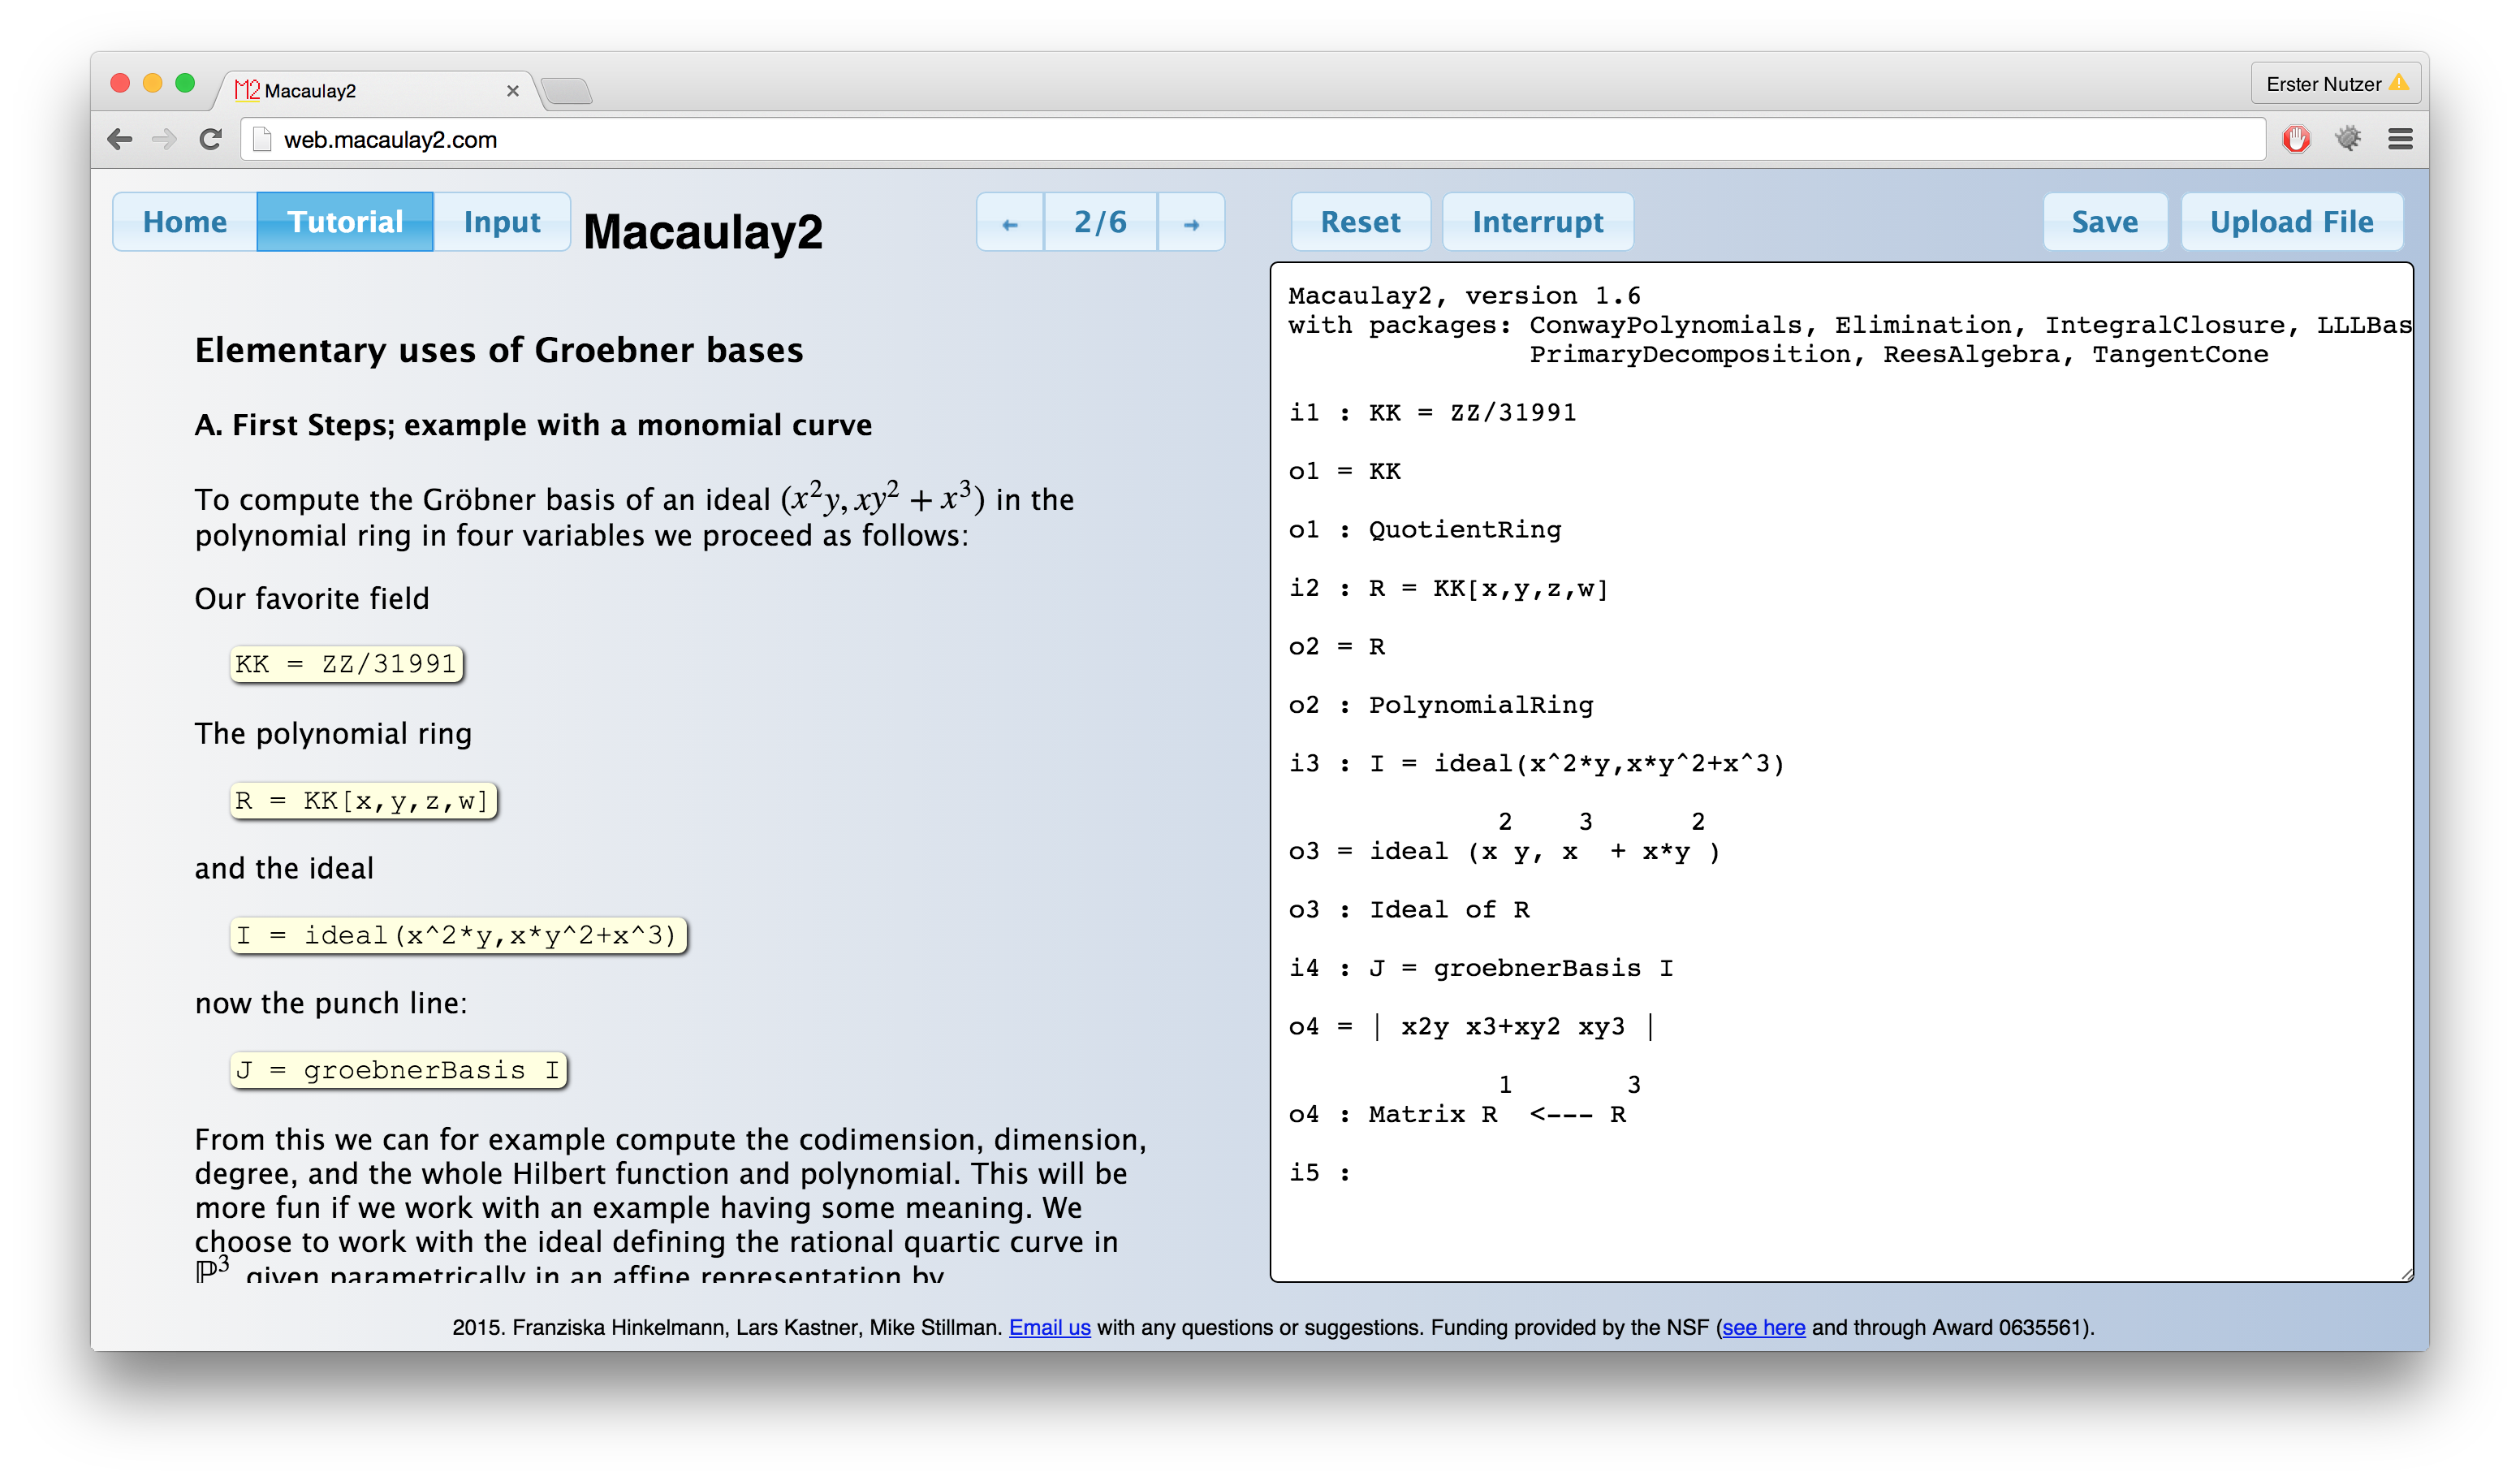
\includegraphics[width=.95\textwidth]{homeWebsite.jpg}
    \caption{A typical view in \tryM2. The left hand
      side shows a tutorial giving an introduction to Gr\"obner
      bases. Text in yellow can be clicked and is then executed by
      Macaulay2 on the server. The complete output of the calculations
      is show on the right hand side. {\it Home, Tutorial, Input} let
      the user change the left hand view, {\it Reset, Interrupt} allow
      to reset and interrupt the Macaulay2 session on the server, {\it
        Save} provides both the input and the output of the current
      session to the user as a text file, and with {\it Upload} one
      can upload files that can then be accessed by \M2.}
    \label{fig:home}
\end{figure}



\tryM2 is an on-line version of \M2 \cite{M2} which
does not require users to download or install the program, and also
does not require users to set up an account and log in.  \tryM2
has the same functionality as the desktop version,
albeit users might have access to less resources
than on their own machine. Users can upload files and
load packages, generate files such as images, and also have
access to other shell commands, such as gfan, 4ti2, and code for
generating images of graphs.

Our primary motivation for creating this web application was to
provide an easy to use experience for classroom and student use.
Having students download and install software such as \M2 is time
consuming and inevitably there are some situations for which this
process fails or takes significant effort to get runnning, e.g., on
some versions of Windows.  The \tryM2 web application is designed to
be able to handle many students at once, and without having the users
need to create accounts or log in.  \tryM2 was used at the Syzygyies
meeting in Berlin in May 2013, with about 70 users.  We would like to point out that the
site is suited not only for beginners, but also for seasoned experts.

We considered off the shelf solutions, such as the Sage
notebook~\cite{sagenotebook}, but decided that we wished for a
lighter-weight solution, and one that did not require users to create
new accounts at a web site.  Nothing available seemed to meet our
needs, hence the current system.

\tryM2 runs under the Chrome, Firefox and Safari web browsers, but not
under Internet Explorer.  On the iPad, it runs under Chrome and
Safari, although it seems that Chrome offers a nicer user experience.
It runs under recent versions of Android ($4.0$ and higher).

In addition to presenting an interface to an instance of \M2
running on a distant server, a number of tutorials to
learn \M2 are provided.  Instructors can create their own
tutorials, and can make them available to their students, as well as
to other \M2 users.  

In Section 2, we describe the basics of using the web application.
Section 3 details how to create and make available your own tutorials.
Providing a program such as \M2 which allows users to
access system resources presents a number of challenges to keep users
from naively or mischievously misusing the system.  In Section 4, we
provide details as to how we structure the application on the server.
In the last section, we describe some of our wish-list items for
improving and extending the system.

The system is open source, and available on github (see \cite{github}).
If you would like more information on using this in your own courses,
or if you have suggestions, please contact one of us.

We would like to thank Charles Boyd, Dan Grayson, Greg Smith, and Benjamin Lorenz for
fruitful discussions on system security and on user interface design.

\section{How to use the website}
The right hand side provides a shell like environment running
Macaulay2. You can type into it, as well as use the arrow keys for
navigating through your command history.

On the left hand side, the user can navigate between {\it Home}, {\it
  Tutorial}, and {\it Input}. {\it Home} shows the table of contents
of tutorials. {\it Tutorial} shows the currently selected
tutorial. Tutorials are interactive and contain executable pieces of
Macaulay2 code that are run by clicking on them. {\it Input} shows a
terminal window in which the user can type {\it Macaulay2} commands and execute them.

All code executed, either by clicking on interactive parts in a
tutorial or by entering code in the {\it Input} window, appears on the
right hand side together with the output from Macaulay2 to those
results.

The {\it Reset} button resets a Macaulay2 session, i.e., restarts 
the \M2 process: it stops any running calculation, deletes all variables, 
unloads all packages, and then reloads the standard packages.

The {\it Interrupt} button stops a running calculation, without
resetting the Macaulay2 session.

\subsection{Features}

The user is free to run all \M2 commands that are available in the
running version. To find the version of \M2 running on the server,
enter and evaluate: {\tt version\#"VERSION"}.  Loading packages is
done using {\tt loadPackage} or {\tt needsPackage}, e.g. {\tt needsPackage "BoijSoederberg"}.  
New packages can be
uploaded to the user's session, by clicking the {\it Upload file}
button. Similarly, any other file, such as text files, that one might
want to manipulate or read data from with \M2, can be uploaded to
the user's session.

%Loading packages is possible, too, with commands
%such as {\tt loadPackage}. If packages are not available, they can be
%uploaded to the users session, by clicking the {\it Upload file}
%%nbutton. Similarly, any other file, such as text files, that one might
%want to manipulate or read data from with Macaulay2 can be uploaded to
%the user's session.

\begin{figure}[htb]
    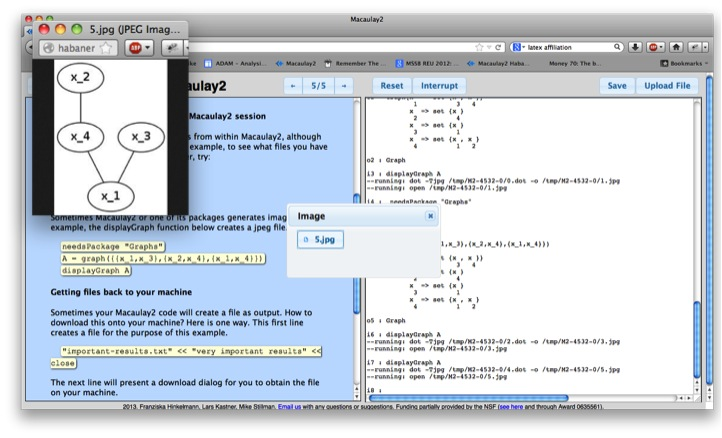
\includegraphics[width=.95\textwidth]{withGraph.jpg}
    \caption{Screenshot of \tryM2 after the user
      generated an image. Some Macaulay2 packages can generate
      graphs. By invoking the command {\tt displayGraph}, the image is
      generated on the server and displayed to the user.}
    \label{fig:graph}
\end{figure}

Results from a session can be retrieved by using the {\it Save}
button, or by using copy and paste. If Macaulay2 generates
images such as graphs, those are presented to the user, see Figure \ref{fig:graph}.

%If the user needs to retrieve
%files that are stored in his session, those can be retrieved by
%executing {\tt open} in the user's session. 

Session are usually kept alive for several days, which allows users to
continue their work next time they access the server, if either they
have not closed their browser, or set the browser to remember their
windows.

\section{Tutorials}
Instructors and other users can create their own tutorials for use with \tryM2. Instructors can email or otherwise distribute an html file with their tutorial to their students or seminar participants. They then can load it into \tryM2 and use it. 

Since it it cumbersome to write the tutorial in the required html format, we provide the \M2 package {\it DocConverter}. It converts a file i  
First, you write your tutorial in \M2's {\it SimpleDoc} format, which includes example \M2 code.
Then, run the \M2 command script {\tt convert} to create an html document. This document has the format required by \tryM2 to be displayed nicely as a tutorial. To load this tutorial into your running {\tt web.macaulay2.com} session use the {\tt Load Tutorial} button at the end of the tutorial list.
Your tutorial will remain locally on your computer and is not uploaded to any server. You can easily delete it from the list by clicking on the close button next to its title. It will also be removed from the list the next time you start your browser. 

Email the html file to your students or provide it on your own website for download. Your students then load this tutorial into their {\tt= web.macaulay2.com} session using the {\tt Load Tutorial} button as well.

The following steps to create a tutorial are also documented in the package {\tt DocConverter}.
\begin{enumerate}
\item Create a tutorial in simpledoc format, say {\tt foo.simpledoc}.  For an example, type into \M2, {\tt viewHelp "DocConverter"}.
\item Use {\tt convert "foo"} to create a file "foo.html".
\item In the {\it Home} screen in \tryM2, click on the {\it Load Tutorial} button, and select this file.
\end{enumerate}

In the case that you do not have access to \M2 on your local machine, you can upload the {\it SimpleDoc} file to the server, convert it there and then download it using the \M2 {\tt open} function.


\section{Internal structure, secure chroots}

The \tryM2 web server runs on a virtual machine on a linux computer on the web.
The server is implemented using {\tt node.js}, and the client
communicates with the server via asynchronous AJAX calls, which often
provide very responsive interaction with the server \cite{nodejs}.

Any user with moderate knowledge of linux can set up their own {\it try Macaulay2}
server.  Detailed directions for doing so are in the github repository \cite{github}.

A major concern is security.
One of the first questions that occurred to us in this context was
whether to offer a sandboxed version of \M2 or \M2 with full
functionality.
We decided on the second alternative, since it seemed
easier to realize and more likely to attract new users.  This lead to
several questions:

\begin{enumerate}
\item A fully functional \M2 also gives the user system access. How does that impact security and how to deal with it?
\item How do we distinguish the users on the system?
\item How can we limit resources to prevent one user from breaking the system? e.g. via fork bombs.
\item How do we clean up after a user has left?
\end{enumerate}

The answer to the second question was to create and delete users on
the fly. Since this implies that the server must be run as root, we
decided to run it inside a virtual machine in order not to compromise
the security of the host system.

Since any system command can be run from inside \M2, we
decided to run M2 inside a `secure chroot' (schroot) \cite{schroot}. To provide full
functionality we mount a full file system inside the schroot. The mounting
happens read only, except that the few folders that \M2 needs write access to are provided with a writable layer.
In the definition of a user specific
schroot there is no root user, so it should not be possible to become
root or execute any command via sudo.

When a user connects to the server the following happens:
\begin{enumerate}
\item A user account on the system is created.
\item A schroot configuration file is created with the above user as only user.
\item Control groups for memory and CPU are created.
\item The schroot is started.
\end{enumerate}

Control groups (cgroups) allow you to restrict the number of CPU
shares and the memory for a process and all its children \cite{cgroups}. When M2 is
executed inside a schroot it is called via {\tt cgexec} with the
cgroups specifically created for this user. Using this technique it is
possible to limit the total consumption of CPU and memory by each
user. Additionally we ensure that the administrator of the virtual
machine always is able to execute any command required for
maintenance, i.e. if the node server is down or has been compromised.

At this point, any Macaulay2 command can be run in this schroot inside the
corresponding cgroups.

User cleanup is done with a combination of shell scripts and the web server itself.

You can find a detailed description how to set up this environment on
\cite{trym2-github} in the file {\tt configuring\_linux.tex}.

\section{The future}

Some important small enhancements that we envision include command
line completion and colorization of \M2 code.  However, an important
design decision is to keep the interface as simple as possible.

The system we have written was designed with \M2 in mind, but 
the entire structure will work for other command line programs such as Singular \cite{singular},
and GAP \cite{GAP4}.  We are currently working on creating a similar server for Singular.
Tutorials for other systems may be created in the same way as \M2 tutorials.

We are excited to receive tutorials that you have developed and would be happy to include them on the website, so that others can profit from your work as well. We plan to develop the feature to upload your tutorials for others as well as a more sophisticated tutorial review process. 

\bibliographystyle{plain}
\bibliography{references}
\end{document}

. What we do?
  . Provide a web-based M2
  . Full featured
  . No creation of accounts needed.
  . No setup time to use in a class setting.  Students can work immediately, with no setup fuss.
  . Tutorials to learn M2 provided.
  . Instructors can create their own tutorials for their students to learn.
  . Also suitable for advanced users.
  . The source is open and on github: any user can create a web-based server
      for others.  Todo: can lock it down to your own self.
  . This runs acceptably on ipad and android, although having a separate 
    keyboard is good.  Future: improve experience on tablets.

  section 2: how to use web Macaulay2, an overview of the features.
  section 3: writing tutorials, making them available.
  section 4: some details about how the server was written and structured.
  section 5: wishlist for additional features.

. Why not other solutions, such as the Sage notebook?
  . need accounts
  . this solution seems more ``lightweight''
